Coding the stored data creates redundancy in the memory. This redundancy is used to serve the requests for reads. This is very efficient in the scenarios where the readrequest have bank conflicts. The redundancy parallalizes the serial access to banks increasing the access speeds, which in turn increases the system efficiency. The previous sections explained the scheme of creating redundancy (or coding scheme). In this section, we use the same coding scheme to create an algorithm for write access to the memory storage. \\
The write requests is issued at a cache miss to the memory controller. The write request composes of $[$Starting Address, Length, Write Data$]$. The memory controller, on the receipt of this request, queues the request in various banks depending on the starting address and length. \\
Let us assume that the priority of read request over write request is $\gamma$. 
The implementation scenario is, we have 8 data banks. We also have 12 shallow(less deep) parity banks. The memory is divided in to two code region. Each code region contains 4 data banks and 6 parity banks. Figure~\ref{fig:code_region} shows the memory layout. The figure shows two coded region having 4 data banks each. 
\begin{figure}[ht!]
\centering
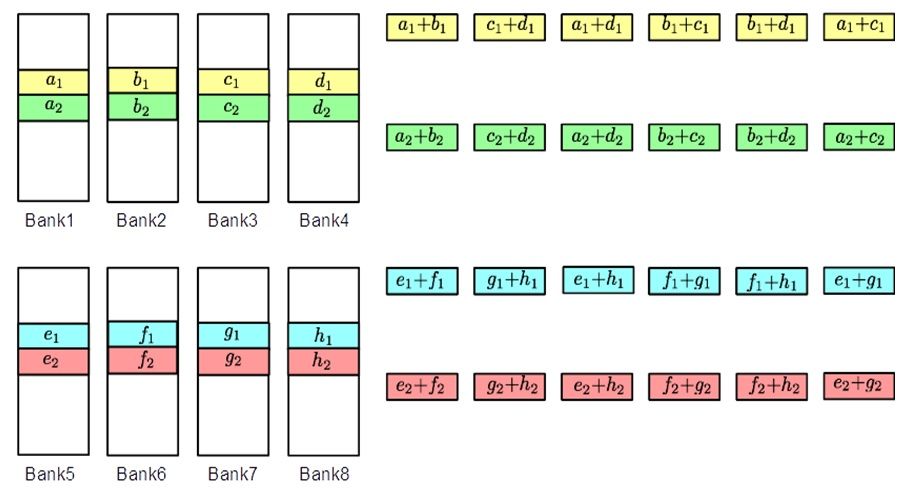
\includegraphics[width=90mm,natwidth=610,natheight=642]{code_region.jpg}
\caption{Memory Bank layout}
\label{fig:code_region}
\end{figure}
When a memory controller receives a write request, it decodes the request and forms $[$address, data$]$ for each bank. The controller then queues each of these request to the respective bank queues. \\
 \\
First Controller algorithm: 
\begin{itemize}
\item Expand the write request.
\item Queue the write request to the memory bank queues.
\end{itemize}
Each data bank has a read and write queue. The second controller forms the access pattern for both the data bank and the parity banks. \\
 \\
Second Controller algorithm: 
\begin{itemize}
\item Reads have higher priority than write. Write Queue's current capacity decides the weight of write access over read access. 
\item Forms the access for each cycle on data and parity banks. 
\item 
\end{itemize}
